\documentclass[11pt]{article}

\usepackage[margin=1in]{geometry}
\usepackage{booktabs}
\usepackage{graphicx}
\usepackage{parskip}
\usepackage{tabularx}
\usepackage{enumitem}
\usepackage{hyperref}

\title{\textbf{Project EDA Report}\\[4pt]
Nocturnal VPR: Dataset and Experiment Diagnostics}
\author{Rhoda Ojetola \and Peter Adeyemo \and Samuel Olusola}
\date{April 24, 2026}

\begin{document}
\maketitle

\section*{Purpose}
This exploratory data analysis (EDA) was designed to answer a simple question before adding more model complexity: \textit{what is actually difficult about our data, and what do the current results suggest about the next useful step?}

The analysis combines:
\begin{itemize}[leftmargin=*]
  \item image statistics for \textbf{GardensPoint} and the \textbf{strict campus dataset},
  \item label and place-coverage analysis for the campus data, and
  \item a comparison of descriptor results already saved in the experiment run folders.
\end{itemize}

\section*{How The EDA Was Run}
The code for this EDA is in \texttt{analysis/project\_eda.py}. It loads the same datasets already used by the benchmark scripts, computes per-image statistics, parses saved experiment result files, and writes plots into \texttt{output\_images/runs/eda/}.

\section*{Question 1: How strong is the day-night appearance gap?}
\textbf{Answer:} The answer depends on the dataset, and that difference matters.

\begin{center}
\begin{tabular}{lccc}
\toprule
\textbf{Split} & \textbf{Brightness Mean} & \textbf{Contrast Mean} & \textbf{Sharpness Mean} \\
\midrule
GardensPoint day & 97.1 & 58.9 & 405.8 \\
GardensPoint night & 127.6 & 69.8 & 718.3 \\
Campus day & 112.0 & 53.5 & 784.2 \\
Campus night & 79.1 & 48.4 & 719.7 \\
\bottomrule
\end{tabular}
\end{center}

\begin{figure}[h!]
\centering
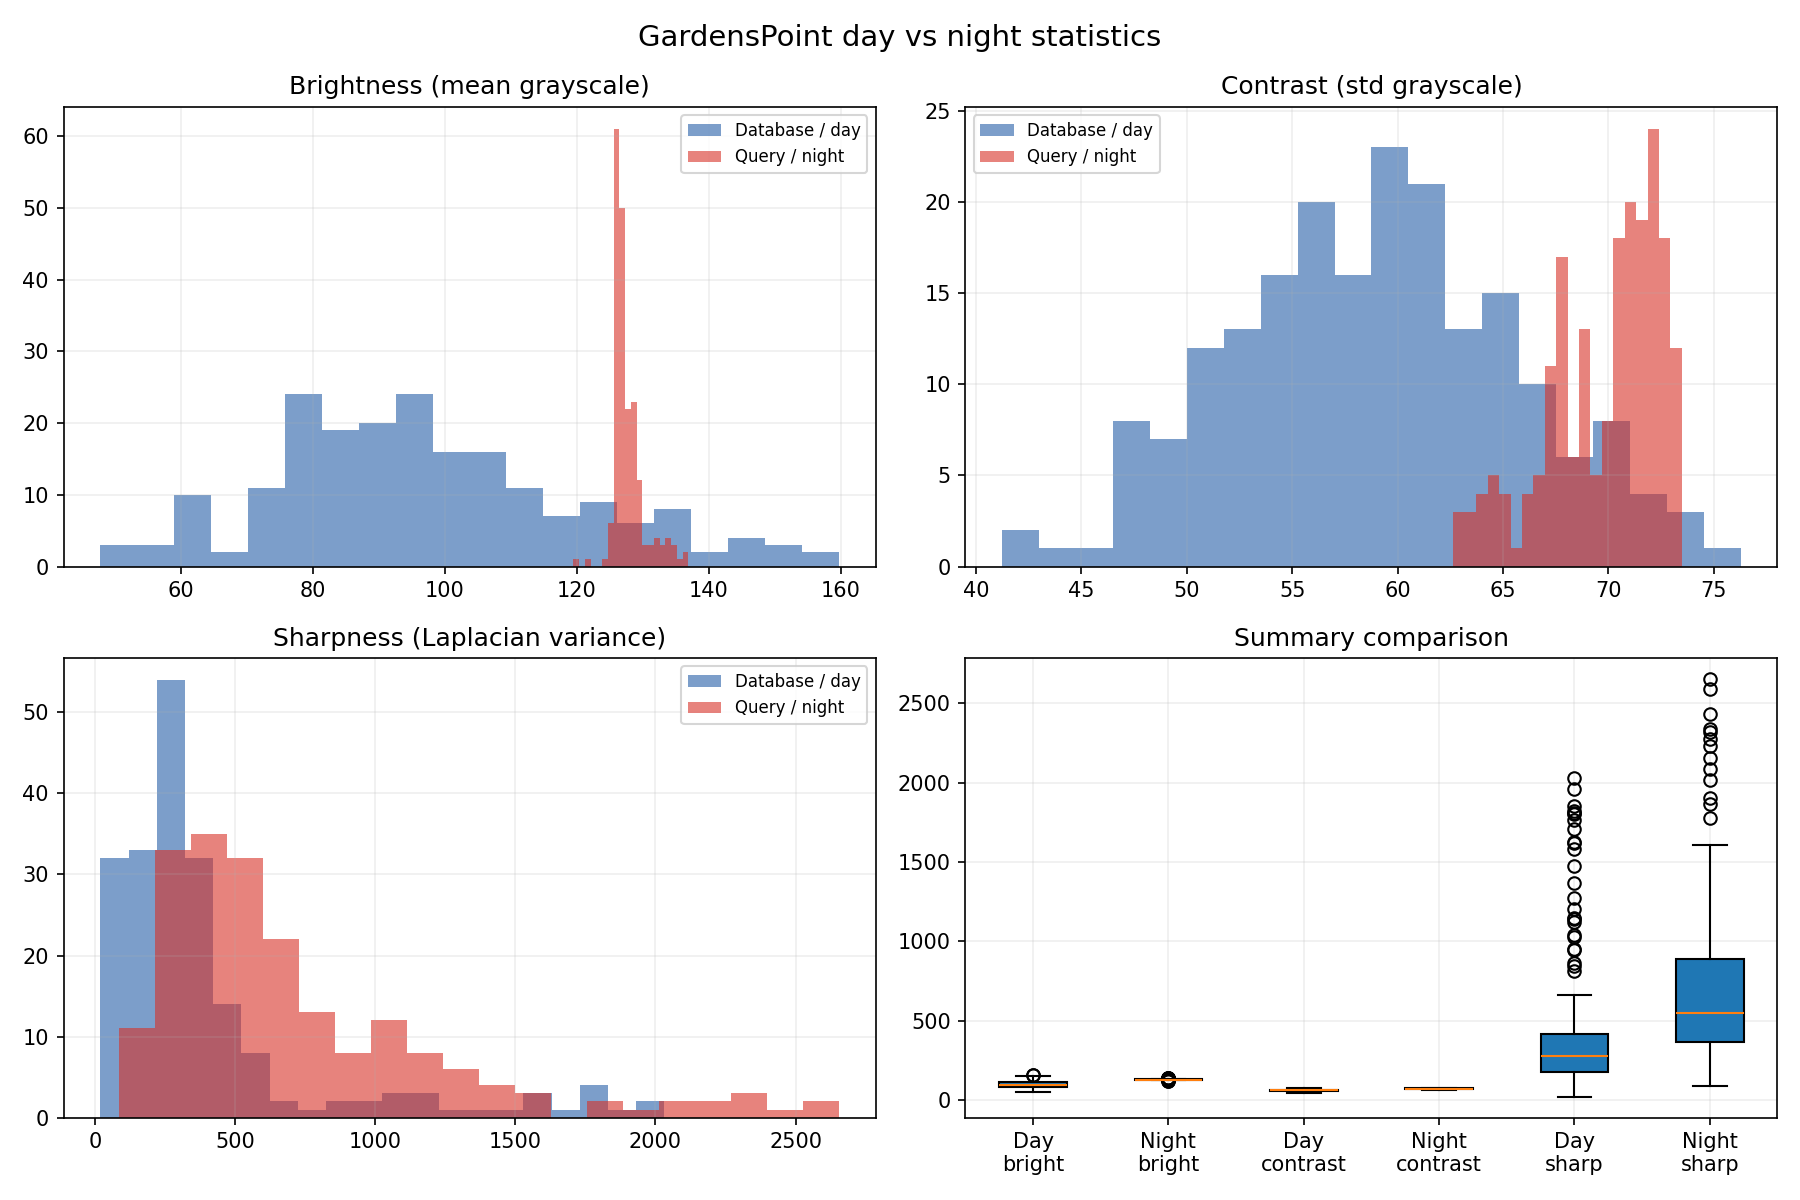
\includegraphics[width=0.86\textwidth]{../../output_images/eda/experiment_diagnostics/gardenspoint_day_night_stats.png}
\caption{GardensPoint day versus night image statistics.}
\end{figure}

\begin{figure}[h!]
\centering
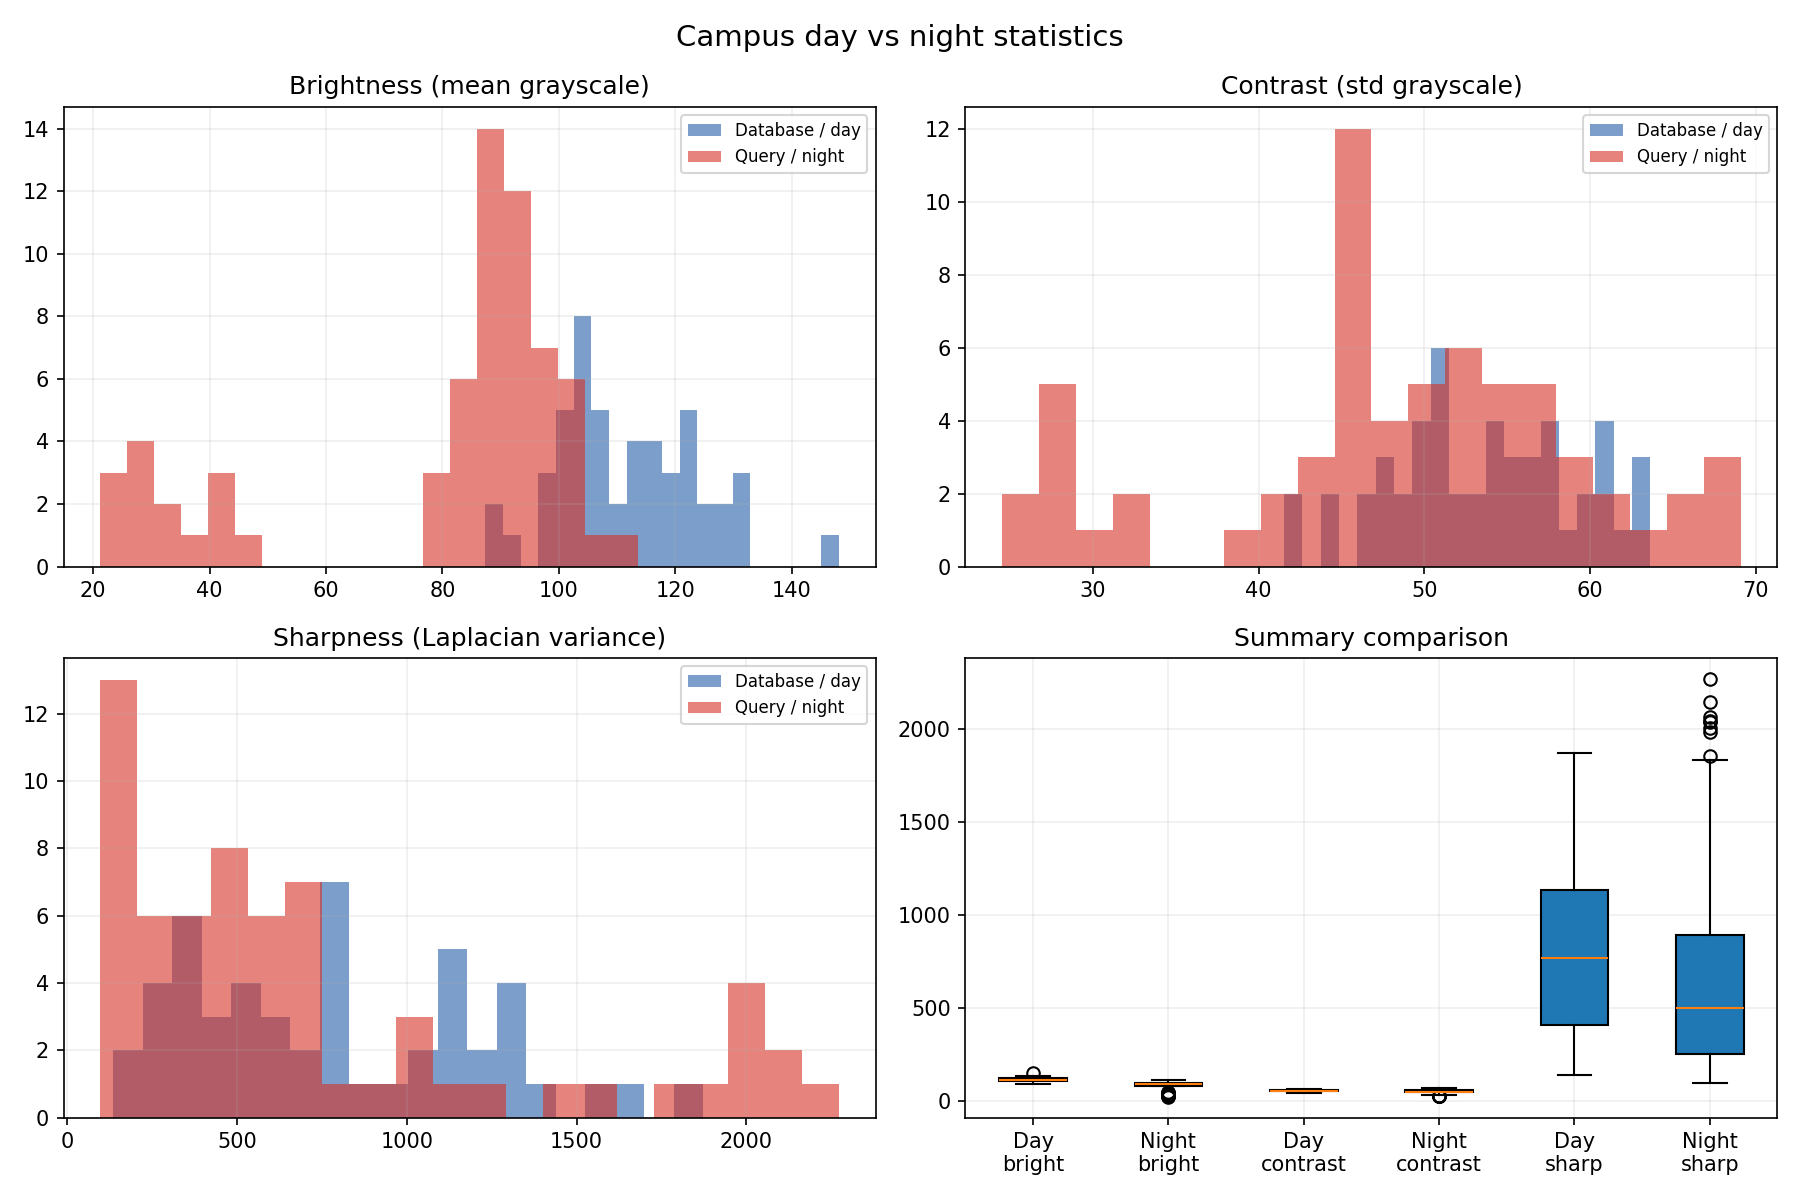
\includegraphics[width=0.86\textwidth]{../../output_images/eda/experiment_diagnostics/campus_day_night_stats.png}
\caption{Campus day versus night image statistics.}
\end{figure}

\textbf{Interpretation.}
\begin{itemize}[leftmargin=*]
  \item On \textbf{GardensPoint}, the night images are on average \textbf{brighter}, more contrasty, and sharper than the day images.
  \item On \textbf{campus}, the night images are clearly \textbf{darker} and slightly lower in contrast than the day images.
  \item Visually, the GardensPoint night frames appear exposure-compensated or over-brightened, which explains why their average intensity is unexpectedly high.
  \item This means the two datasets do not represent the same kind of night-time difficulty. GardensPoint is still useful as a controlled benchmark, but it does not fully reflect the darker and noisier campus setting.
\end{itemize}

\section*{Question 2: Is the strict campus protocol inherently hard?}
\textbf{Answer: Yes.} The strict campus setup is hard not only because of descriptor quality, but also because many queries are treated as no-match cases.

\begin{figure}[h!]
\centering
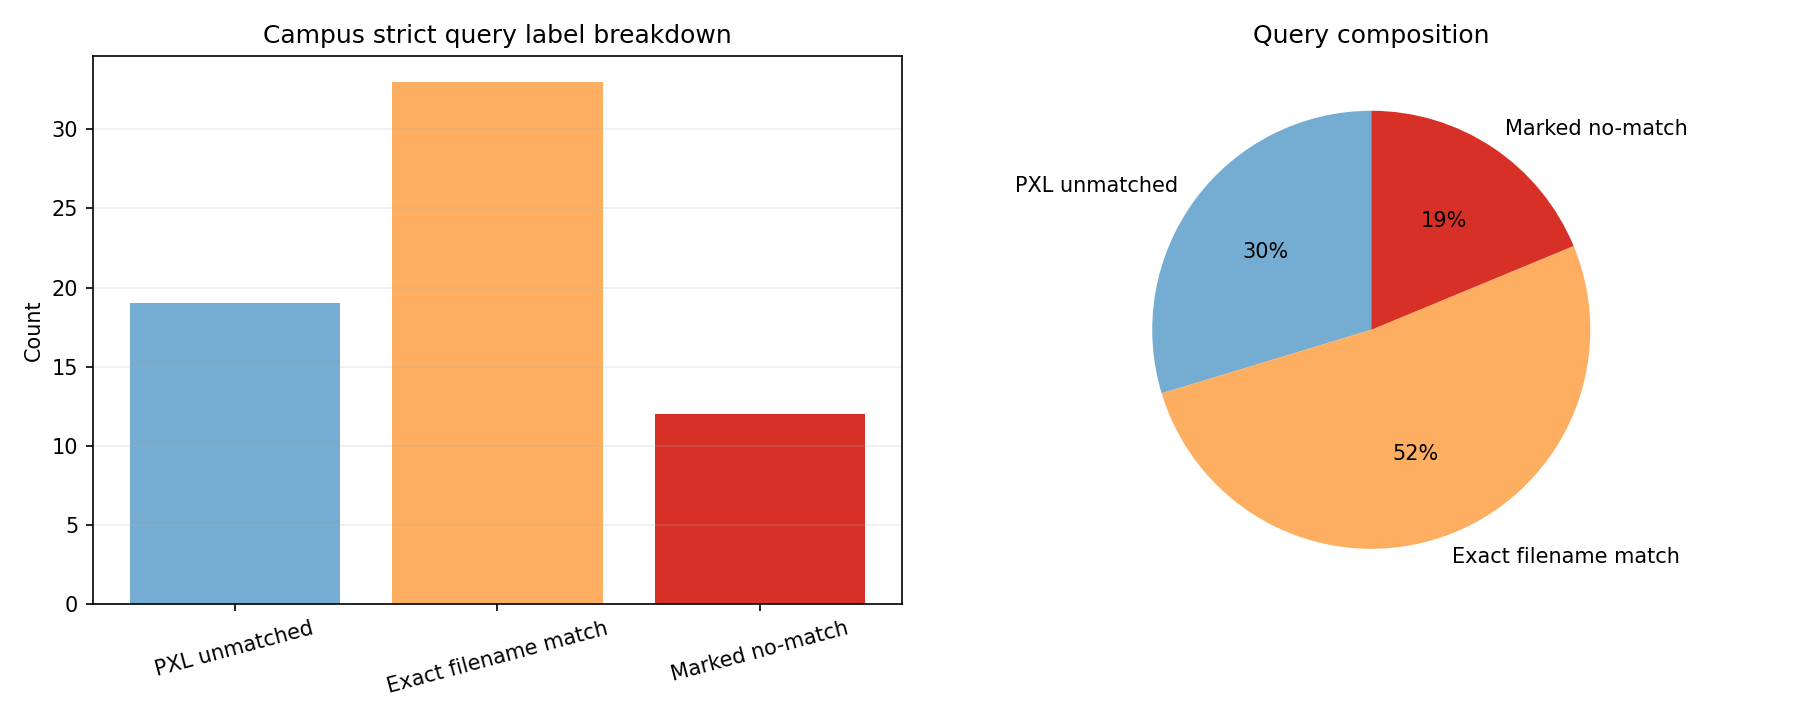
\includegraphics[width=0.82\textwidth]{../../output_images/eda/experiment_diagnostics/campus_label_breakdown.png}
\caption{Strict campus query composition.}
\end{figure}

The strict campus query set contains:
\begin{itemize}[leftmargin=*]
  \item \textbf{33} exact filename matches,
  \item \textbf{12} queries explicitly marked as no-perfect-match, and
  \item \textbf{19} \texttt{PXL\_*} phone images with no strict day counterpart.
\end{itemize}

So nearly half of the strict campus query set is not a simple one-to-one retrieval problem. This helps explain why thresholded precision-style metrics remain low even when top-\(k\) retrieval is strong. These \texttt{PXL\_*} images are intentionally kept because they act as hard no-match queries in the strict setting.

\section*{Question 3: Is place coverage balanced across the campus walk?}
\textbf{Answer: Not really.} The campus place-level annotations reveal an uneven distribution of visual evidence.

\begin{figure}[h!]
\centering
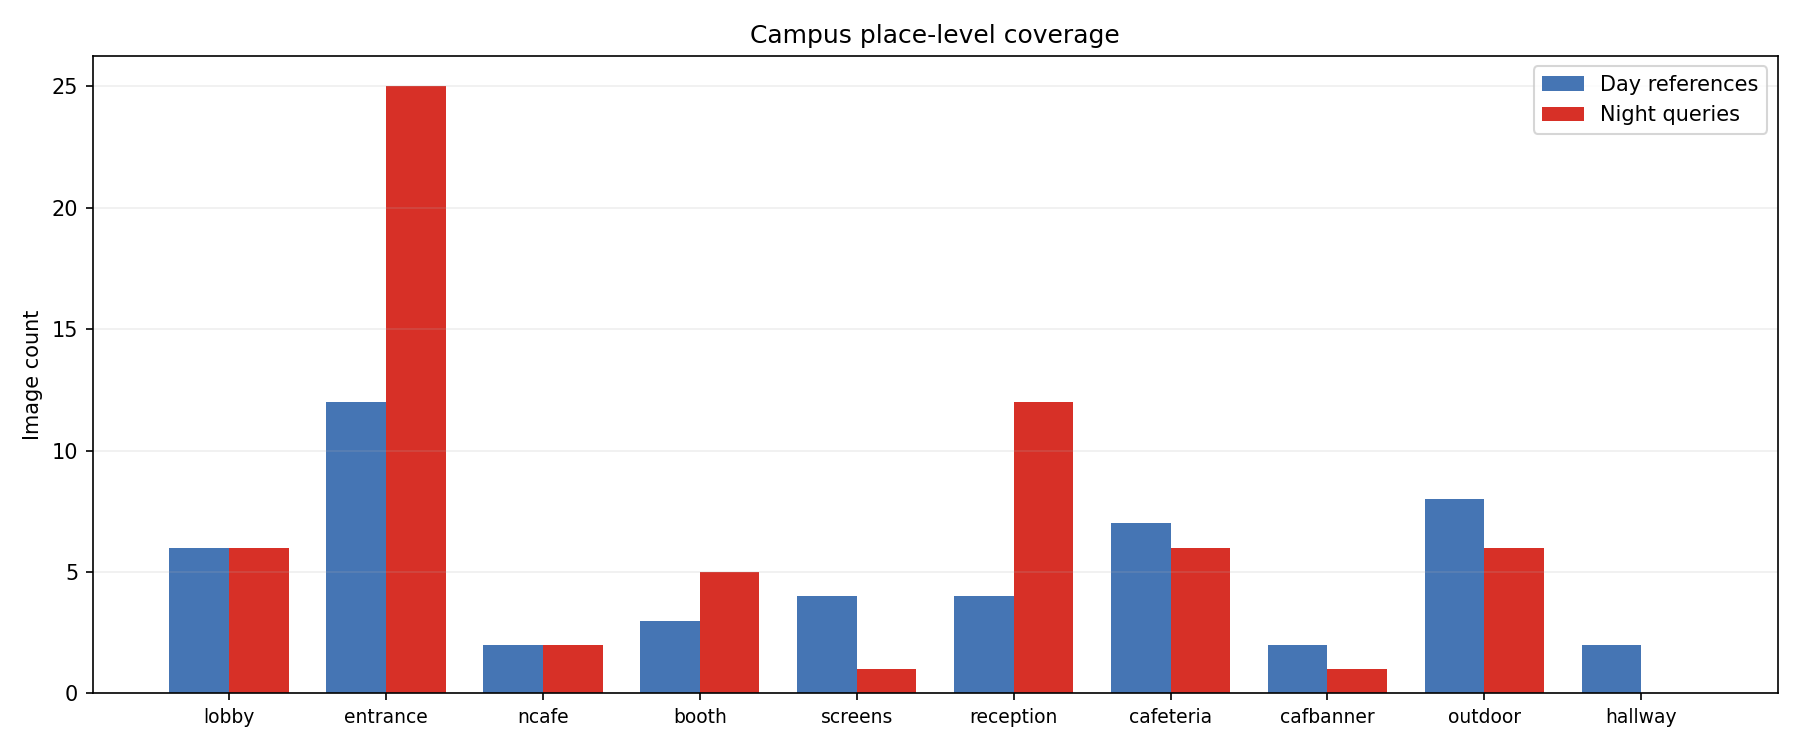
\includegraphics[width=0.95\textwidth]{../../output_images/eda/experiment_diagnostics/campus_place_coverage.png}
\caption{Place-level day and night coverage across the campus walk.}
\end{figure}

\textbf{Main observations.}
\begin{itemize}[leftmargin=*]
  \item The largest night bucket is \textbf{\texttt{entrance}} with \textbf{25} night images.
  \item Some places have very little support, such as \texttt{ncafe} and \texttt{cafbanner}.
  \item \texttt{hallway} has day images but no confident night counterpart in the place-level rematch.
\end{itemize}

This uneven coverage means that some locations are much more likely to dominate the matching statistics than others. When a descriptor performs well, part of that success may come from repeatedly seeing the same overrepresented place types rather than solving every place equally well.

\section*{Question 4: Which descriptors currently look strongest?}
\textbf{Answer:} The current evidence supports modern VPR descriptors, but their relative strengths differ by metric.

\begin{figure}[h!]
\centering
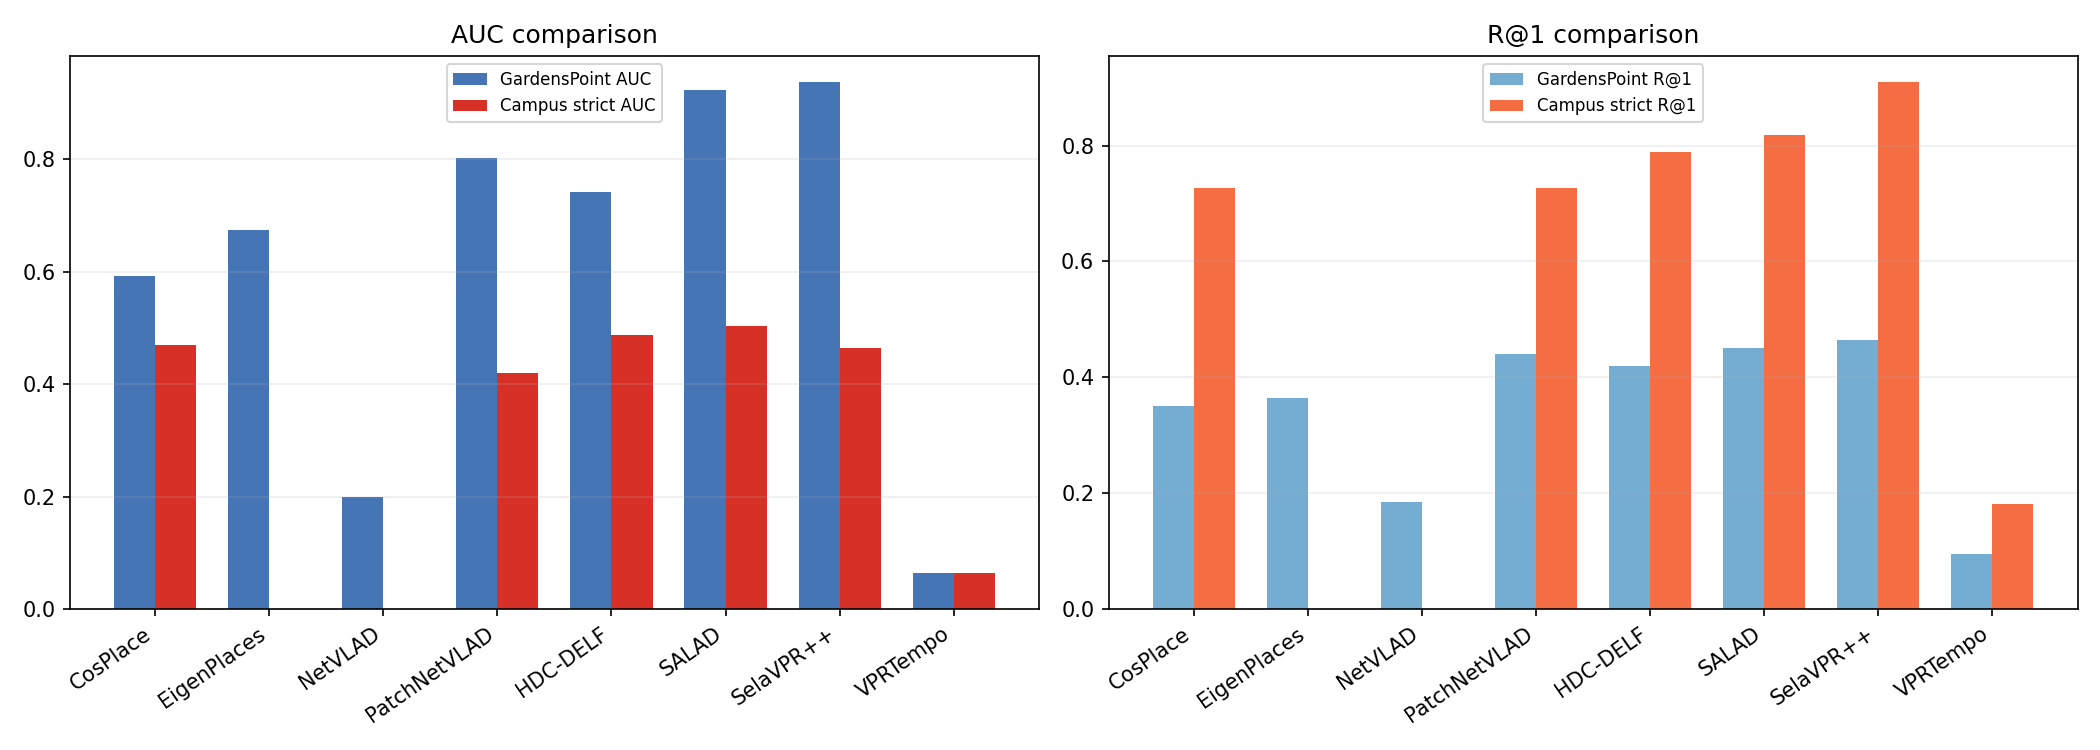
\includegraphics[width=0.95\textwidth]{../../output_images/eda/experiment_diagnostics/descriptor_comparison.png}
\caption{AUC and R@1 comparison across the saved GardensPoint and strict campus runs.}
\end{figure}

From the saved runs:
\begin{itemize}[leftmargin=*]
  \item \textbf{GardensPoint AUC}: best is \textbf{SelaVPR++} at \textbf{0.937}.
  \item \textbf{GardensPoint R@1}: best is \textbf{SelaVPR++} at \textbf{0.465}.
  \item \textbf{Strict campus AUC}: best is \textbf{SALAD} at \textbf{0.504}.
  \item \textbf{Strict campus R@1}: best is \textbf{SelaVPR++} at \textbf{0.909}.
\end{itemize}

\textbf{Interpretation.}
\begin{itemize}[leftmargin=*]
  \item \textbf{SALAD} and \textbf{SelaVPR++} are the most promising current descriptors.
  \item \textbf{CosPlace} remains a strong and simpler baseline.
  \item \textbf{VPRTempo} transfers poorly in this setup, which is consistent with the fact that the checkpoint we tested is a specialized demo model rather than a universal descriptor.
\end{itemize}

\section*{Question 5: What does this imply for the project?}
\textbf{Answer:} The EDA supports the current project direction.

\begin{enumerate}[leftmargin=*]
  \item \textbf{Descriptor exploration is justified.} The descriptor choice clearly changes performance in a meaningful way.
  \item \textbf{GardensPoint is still worth keeping.} It remains the right controlled day-to-night benchmark, even though it is not identical to campus.
  \item \textbf{The campus challenge is broader than descriptor weakness alone.} It includes harder no-match composition, small-data imbalance, and viewpoint ambiguity.
  \item \textbf{The next useful step is not random model complexity.} The most sensible next phase is to keep the strong descriptors and add lightweight improvements for rejection and temporal stability, such as CLAHE, sequence matching, or other temporal cues.
\end{enumerate}

\section*{Conclusion}
The EDA clarifies an important point: \textbf{our benchmark and deployment datasets represent different kinds of night-time difficulty}. GardensPoint tests controlled day-to-night retrieval, while the strict campus set adds darker imagery, harder no-match cases, and uneven place coverage. This makes the current results easier to trust and easier to interpret. The strongest descriptors so far are SALAD and SelaVPR++, and the remaining gap is increasingly about deployment realism rather than only about retrieval quality.

\end{document}
